\documentclass{article}
\usepackage{fancyhdr}

% Set up the custom footer
\pagestyle{fancy}
\fancyfoot[R]{\thepage} % Centered page number in footer
\fancyfoot[C]{\textbf{License:} CC-BY.\textbf{Copyright:} Andree \& Degoot, 2024 }
\usepackage{tikz}
\usetikzlibrary{arrows.meta, positioning}
\usepackage{amsmath}
\author{Andree Valle Campos and Abdoelnaser M Degoot \\ Epiverse-TRACE Team @ LSHTM }
\title{Simple Introduction to Mathematical Modelling of Infectious Diseases}
\begin{document}
\maketitle

\section{Introduction}
This document aims to assess  your understanding of the fundamental 
principles of mathematical modeling while guiding you in constructing models using 
a simple SEIR framework for infectious disease outbreaks. 
 
 \textbf{Note: Please fill in the blanks.}

\section{SEIR Model}

 In the  SEIR model, we have four compartments (\( S \), \( E \), \( I \), \( R \)):

\begin{itemize}
    \item \( S \) stands for \underline{\hspace{2cm}}, meaning \underline{\hspace{3cm}}.
The parameter that explains the transition from  (\( S \)) compartment 
to  (\( E \)) compartment is \underline{\hspace{6cm}}.
\item \(E\) stands for \underline{\hspace{2cm}}, meaning that it can 
    \underline{\hspace{3cm}}. 
    
    The rate that explains the transition from  (\( E \)) to  (\( R \)) is the rate of \underline{\hspace{6cm}}.
    
    \item \( I \) stands for \underline{\hspace{2cm}}, meaning that it can 
    \underline{\hspace{3cm}}.
    The rate that explains the transition from  (\( I \)) to  (\( R \)) is the rate of \underline{\hspace{6cm}}.
    
    \item \( R \) stands for \underline{\hspace{3cm}}. This compartment includes those who have ceased to be infectious and acquire immunity against infection, regardless of the clinical course.
\end{itemize}

\section{\( R_0 \)}
\( R_0 \) helps project the potential 
size of an epidemic and calculate the herd immunity threshold.
It is defined as the average number of \underline{\hspace{2cm}} secondary cases 
generated from a primary case in a completely 
\underline{\hspace{3cm}} population. 

\section{\( R_t \)}
\( R_t \) 
helps monitor the progress of the epidemic 
When the population is no longer \underline{\hspace{2cm}}, the instantaneous 
reproduction number \( R_t \) is used. This is defined as the average number 
of s\underline{\hspace{2cm}} in a population composed of 
\underline{\hspace{2cm}} and non-\underline{\hspace{2cm}} individuals at time \( t \).

\section{A Diagram for Measles outbreak}

Below is a typical SEIR model with demography (births and deaths). This is a simple 
model applicable to person-to-person infections in a homogeneously mixing population.
Please carefully observe the model and examine the interactions with the equations 
in section \ref{eqs}.  Use color codes or arrows to relate the diagram to the equations.


\begin{center}
    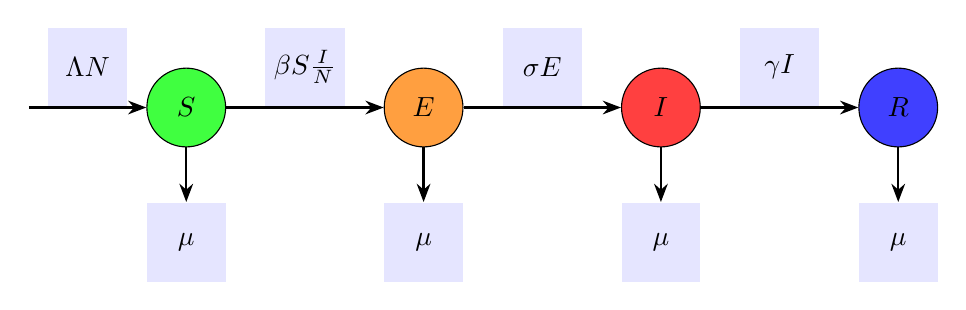
\begin{tikzpicture}[
        node distance=2cm, 
        every node/.style={fill=blue!10, draw, minimum size=1cm, text centered},
        arrow/.style={-Stealth, thick}
    ]
    
    % Nodes
    \node [circle, fill=green!75](S) {$S$};
    \node [circle, fill=orange!75](E) [right=of S] { $E$};
    \node [circle, fill=red!75](I) [right=of E] {$I$};
    \node [circle, fill=blue!75](R) [right=of I] {$R$};
    
    % Arrows for transitions
    \draw[arrow] (S) -- node[above, draw=none] {$\beta S  \frac{I}{N}$} (E);
    \draw[arrow] (E) -- node[above, draw=none] {$\sigma  E$} (I);
    \draw[arrow] (I) -- node[above, draw=none] {$\gamma  I$} (R);
    
    % Natural birth and death rates
    \draw[arrow] (-2,0.0) -- node[above, draw=none] {$\Lambda N$} (S);
    \draw[arrow] (S) -- +(0,-1.2) node[below, draw=none] {$\mu$};
    \draw[arrow] (E) -- +(0,-1.2) node[below, draw=none] {$\mu$ };
    \draw[arrow] (I) -- +(0,-1.2) node[below, draw=none] {$\mu$ };
    \draw[arrow] (R) -- +(0,-1.2) node[below, draw=none] {$\mu$};
    
    \end{tikzpicture}
\end{center}

Where:
\begin{itemize}
    \item \( \beta \): Transmission rate
    \item \( \sigma \): Rate of progression from exposed to infectious
    \item \( \gamma \): Recovery rate
    \item \( \mu \): Death rate (natural death rate)
    \item \( N \): Total population size, \( N = S + E + I + R \).
\end{itemize}

 The parameter $\beta$ is derived from the multiplication of $p$
  and $c$, where $p$ is the probability of transmission during contact, and $c$ 
  is the contact rate, defined as the average number of contacts per unit of time. 

\section{Equations}\label{eqs}
Note that in the diagram, arrows entering compartments are expressed as positive 
terms in the equations, while arrows exiting compartments are represented with negative terms.
Based on the above diagram,deduce the following equations that describe this system:

\section*{Compartment Equations}

\begin{itemize}
    \item \textbf{S compartment:}
    \[
    \frac{dS}{dt} = 
    \]
    
    \item \textbf{E compartment:}
    \[
    \frac{dE}{dt} = 
    \]
    \item \textbf{I compartment:}
    \[
    \frac{dI}{dt} = \
    \]
    
    \item \textbf{R compartment:}
    \[
    \frac{dR}{dt} =
    \]
\end{itemize}

\section{Computing $R_0$}
The expression for the basic reproduction number ($R_0$) in the above system  is given by:

\begin{equation*} R_0 = \frac{\mu}{(\mu + \sigma)} \frac{\beta}{(\mu + \gamma)}. \end{equation*}

To calculate the $R_0$ value for given parameter values,  write an R function 
called Measles$R_0$ that implements this formula. The function will use the following parameter values:

    \begin{itemize}
        \item $\mu = \frac{1}{75}$ (natural mortality rate)
        \item $\sigma = \frac{1}{10}$ (rate of progression from the exposed to the infectious stage)
        \item $\gamma = 1/8$ (recovery rate)
        \item $\beta = 1.8$ (transmission rate)
    \end{itemize}
Then compute the final size of such epidemic.
\end{document}